\textcolor{blue}{Problem 2}

8.3 Uniformly distributed noise. Let the input random variable $X$ to a channel be uniformly distributed over the interval $-\frac{1}{2} \leq x \leq+\frac{1}{2}$. Let the output of the channel be $Y=X+Z$, where the noise random variable is uniformly distributed over the interval $-a / 2 \leq z \leq$ $+a / 2$.

(a) Find $I(X ; Y)$ as a function of $a$.

(b) For $a=1$ find the capacity of the channel when the input $X$ is peak-limited; that is, the range of $X$ is limited to $-\frac{1}{2} \leq x \leq$ $+\frac{1}{2}$. What probability distribution on $X$ maximizes the mutual information $I(X ; Y)$?

(c) (Optional) Find the capacity of the channel for all values of $a$, again assuming that the range of $X$ is limited to $-\frac{1}{2} \leq x \leq+\frac{1}{2}$.

\textcolor{blue}{Solution}

From the discription, we can get that
$$X\sim\text{Unif}\left(-\frac{1}{2},\frac{1}{2}\right), f_X(x)=1,x\in\left[-\frac{1}{2},\frac{1}{2}\right]$$
$$Z\sim\text{Unif}\left(-\frac{a}{2},\frac{a}{2}\right), f_Z(z)=\frac{1}{a},z\in\left[-\frac{a}{2},\frac{a}{2}\right]$$
So we have:
$$f_Y(y) = \int_{-\infty}^{+\infty}\Pr\left(X=z-y|Z=z\right)\Pr(Z=z)dz=\int_{-\infty}^{+\infty}f_X(y-z)f_Z(z)dz = f_X * f_Z $$
Where $*$ denotes the convolution operation.

And since $f_X,f_Z$ could be regarded as two rectangle signals, so their convolution if the sum of their products in the intersection range. It could be easier to compute with slicing window. And since the range of $Z$ is $[-\frac{a}{2},\frac{a}{2}]$, which means that $a>0$, so we have: \\
1. If $a = 1$: \\
$$f_Y(y)=\begin{cases}
y+1, & -1 \leq y < 0 \\
1-y, & 0 \leq y \leq 1 \\
0, &\text{otherwise}
\end{cases}$$

2. If $0<a<1$: \\
$$f_Y(y)=\begin{cases}
\frac{1}{a}\left(y+\frac{1}{2}+\frac{a}{2}\right), & -\frac{1}{2}-\frac{a}{2}\leq y<-\frac{1}{2}+\frac{a}{2} \\
1, & -\frac{1}{2}+\frac{a}{2}\leq y<\frac{1}{2}-\frac{a}{2} \\
-\frac{1}{a}\left(y-\frac{1}{2}-\frac{a}{2}\right), & \frac{1}{2}-\frac{a}{2}\leq y\leq\frac{1}{2}+\frac{a}{2} \\
0, & \text{otherwise}
\end{cases}$$

3. If $a>1$: \\
$$f_Y(y)=\begin{cases}
\frac{1}{a}\left(y+\frac{1}{2}+\frac{a}{2}\right), & -\frac{1}{2}-\frac{a}{2}\leq y<\frac{1}{2}-\frac{a}{2} \\
\frac{1}{a}, & \frac{1}{2}-\frac{a}{2}\leq y<-\frac{1}{2}+\frac{a}{2} \\
-\frac{1}{a}\left(y-\frac{1}{2}-\frac{a}{2}\right), & -\frac{1}{2}+\frac{a}{2}\leq y\leq\frac{1}{2}+\frac{a}{2} \\
0, & \text{otherwise}
\end{cases}$$

And before we compute the mutual information, we calculate a mostly used calculation first:
\begin{align*}
I &= \int_{0}^{1}t\ln t \dt \\
&= \left. \left[t\cdot \left(t\ln t\right)\right]\right|_{0}^{1}-\int_{0}^{1} t \text{\ d}\left(t\ln t\right) \\
&= 0 - 0 - \int_{0}^{1} t \cdot \left(1+\ln t\right) \dt \\
&= -\int_{0}^{1} t \dt - \int_{0}^{1} t\ln t \dt \\
&= -\frac{1}{2} - I \\
\Rightarrow I &= -\dfrac{1}{4}
\end{align*}
i.e. we have proved that
$$I=\int_{0}^{1}t\ln t \dt = -\dfrac{1}{4}$$

(a) Combined with previous discussion, we can get the mutual information:
\begin{align*}
I(X;Y) &= h(Y)-h(Y|X) \\
&= h(Y)-h(Z|X) \qquad \text{(Since $Y=X+Z$)} \\
&= h(Y)-h(Z) \qquad\quad\ \text{(Since $Z\perp X$)}
\end{align*}
And since $Z\sim \text{Unif}\left(-\dfrac{a}{2},\dfrac{a}{2}\right)$, we have:
$$ h(Z) = -\int_{-\frac{a}{2}}^{\frac{a}{2}}\dfrac{1}{a}\ln\left(\dfrac{1}{a}\right) \dz = a\cdot \dfrac{1}{a}\cdot \ln a = \ln a \ \ \text{nats}$$
So we need to compute the entropy of $Y$: \\
1. If $a=1$:
\begin{align*}
h(Y) &= -\int_{-1}^{0}(y+1)\ln(y+1) \dy - \int_{0}^{1}(1-y)\ln(1-y) \dy \\
&= -\int_{0}^{1}x\ln x \dx - \int_{1}^{0}t\ln t (-1) \dt \qquad \text{(Let $x=y+1, t=1-y$)} \\
&= -2I \\
&= \dfrac{1}{2} \ \ \text{nat}
\end{align*}

2. If $0<a<1$:
\begin{align*}
h(Y) &= -\int_{-\frac{1}{2}-\frac{a}{2}}^{-\frac{1}{2}+\frac{a}{2}}\dfrac{1}{a}\left(y+\frac{1}{2}+\frac{a}{2}\right)\ln\left(\dfrac{1}{a}\left(y+\frac{1}{2}+\frac{a}{2}\right)\right) \dy - \int_{-\frac{1}{2}+\frac{a}{2}}^{\frac{1}{2}-\frac{a}{2}}1 \ln 1 \dy \\
&\quad - \int_{\frac{1}{2}-\frac{a}{2}}^{\frac{1}{2}+\frac{a}{2}} \left(-\dfrac{1}{a}\left(y-\frac{1}{2}-\frac{a}{2}\right)\right)\ln\left(-\dfrac{1}{a}\left(y-\frac{1}{2}-\frac{a}{2}\right)\right) \dy \\
&= -a\int_{0}^{1}x\ln x \dx + a\int_{1}^{0}t\ln t\dt \qquad \text{(Let $x=\dfrac{1}{a}\left(y+\frac{1}{2}+\frac{a}{2}\right), t=-\dfrac{1}{a}\left(y-\frac{1}{2}-\frac{a}{2}\right)$)} \\
&= -a\cdot 2I \\
&= \dfrac{a}{2} \ \ \text{nats}
\end{align*}

3. If $a>1$:
\begin{align*}
h(Y) &= -\int_{-\frac{1}{2}-\frac{a}{2}}^{\frac{1}{2}-\frac{a}{2}}\dfrac{1}{a}\left(y+\frac{1}{2}+\frac{a}{2}\right)\ln\left(\dfrac{1}{a}\left(y+\frac{1}{2}+\frac{a}{2}\right)\right) \dy - \int_{\frac{1}{2}-\frac{a}{2}}^{-\frac{1}{2}+\frac{a}{2}}\dfrac{1}{a}\ln\left(\dfrac{1}{a}\right) \dy \\
&\quad - \int_{-\frac{1}{2}+\frac{a}{2}}^{\frac{1}{2}+\frac{a}{2}} \left(-\dfrac{1}{a}\left(y-\frac{1}{2}-\frac{a}{2}\right)\right)\ln\left(-\dfrac{1}{a}\left(y-\frac{1}{2}-\frac{a}{2}\right)\right) \dy \\
&= -\int_{0}^{1}\left(\dfrac{1}{a}x\right)\ln \left(\dfrac{1}{a}x\right) \dx - \left(\dfrac{1}{a}\right)\ln \left(\dfrac{1}{a}\right)\cdot (a-1) - \int_{1}^{0}\left(\dfrac{1}{a}t\right)\ln \left(\dfrac{1}{a}t\right)(-1)\dt \\
&\qquad (\text{Let } x=y+\frac{1}{2}+\frac{a}{2}, t=-\left(y-\frac{1}{2}-\frac{a}{2}\right)) \\
&= 2\left(\dfrac{\ln a}{a}\int_0^1 x \dx - \dfrac{1}{a}\int_0^1 x\ln x \dx\right) + \dfrac{\ln a}{a}(a-1) \\
&= \ln a + \dfrac{1}{2a} \ \ \text{nats}
\end{align*}

So above all, we have:
$$I(X;Y) = \begin{cases}
\frac{1}{2} \text{ nat}, & a=1 \\
\frac{a}{2}-\ln a \text{ nats}, & 0<a<1 \\
\frac{1}{2a} \text{ nats}, & a>1
\end{cases}$$


(b) Lemma: Among all distributions in the range $[a,b]$, the uniform distribution Unif$(a,b)$ has the highest entropy. \\
Let $X_1\sim\text{Unif}(a,b)$ with PDF $u(x)=\dfrac{1}{b-a},x\in[a,b]$, and $X_2$ be another random variable with PDF $f(x)$ in the same range. We have:
$$h(X_1)=-\int_{a}^{b}u(x)\ln u(x) \dx = \ln(b-a) \ \ \text{nats}$$
Then we have:
\begin{align*}
0 &\leq D\left(f\|u\right) \\
&= \int_{a}^{b}f(x)\ln \dfrac{f(x)}{u(x)} \dx \\
&= \int_{a}^{b}f(x)\ln f(x) \dx + \int_{a}^{b}f(x)\ln u(x) \dx \\
&= \ln(b-a) - h(X_2) \\
&= h(X_1) - h(X_2)
\end{align*}
So we have proved that $h(X_1)\geq h(X_2)$, if and only if $f(x)=u(x)$. \\
Since when $a=1$, $I(X;Y)=h(Y)-\ln a = h(Y)$. To reach the capacity, i.e. the highest mutual information, we need to maximize the entropy of $Y$, i.e. construct $p(x)$ to make $Y\sim \text{Unif}\left(-1,1\right)$. \\
We can construct that
$$X=\begin{cases}
-\frac{1}{2}, & \text{w.p. } \frac{1}{2} \\
\frac{1}{2}, & \text{w.p. } \frac{1}{2}
\end{cases}$$
Then we have:
$$f_Y(y)=\sum_{x}f_{Y|X}(y|x)p(X=x)=\sum_{z}f_Z(y-x)p(X=x)$$
When $y\in[-1,0]$:
$$\left.\begin{array}{l}
\text{if } X=-\dfrac{1}{2}\Rightarrow y-x\in\left[-\frac{1}{2},\frac{1}{2}\right]\Rightarrow f_Z(y-x)=1 \\
\text{if } X=\dfrac{1}{2}\Rightarrow y-x\in\left[-\frac{3}{2},-\frac{1}{2}\right]\Rightarrow f_Z(y-x)=0
\end{array}\right\} \Rightarrow f_Y(y)=\dfrac{1}{2}$$
And when $y\in[0,1]$:
$$\left.\begin{array}{l}
\text{if } X=-\dfrac{1}{2}\Rightarrow y-x\in\left[\frac{1}{2},\frac{3}{2}\right]\Rightarrow f_Z(y-x)=0 \\
\text{if } X=\dfrac{1}{2}\Rightarrow y-x\in\left[-\frac{1}{2},\frac{1}{2}\right]\Rightarrow f_Z(y-x)=1
\end{array}\right\} \Rightarrow f_Y(y)=\dfrac{1}{2}$$

So above all, we have proved that in such construction, $Y\sim\text{Unif}\left(-1,1\right)$, and $C=\max\limits_{p(x)}I(X;Y)=1 \ \text{bit}$.


(c) Let $F(x)$ be the CDF of $X$, similarly to the discussion in the beginning, we have: \\
1. If $0<a<1$: \\
$$f_Y(y)=\begin{cases}
\frac{1}{a}F\left(y+\frac{a}{2}\right), & -\frac{1}{2}-\frac{a}{2}\leq y<-\frac{1}{2}+\frac{a}{2} \\
\frac{1}{a}\left[F\left(y+\frac{a}{2}\right) - F\left(y-\frac{a}{2}\right) \right], & -\frac{1}{2}+\frac{a}{2}\leq y<\frac{1}{2}-\frac{a}{2} \\
\frac{1}{a}\left[1-F\left(y-\frac{a}{2}\right)\right], & \frac{1}{2}-\frac{a}{2}\leq y\leq\frac{1}{2}+\frac{a}{2} \\
0, & \text{otherwise}
\end{cases}$$

2. If $a>1$: \\
$$f_Y(y)=\begin{cases}
\frac{1}{a}F\left(y+\frac{a}{2}\right), & -\frac{1}{2}-\frac{a}{2}\leq y<\frac{1}{2}-\frac{a}{2} \\
\frac{1}{a}, & \frac{1}{2}-\frac{a}{2}\leq y<-\frac{1}{2}+\frac{a}{2} \\
-\frac{1}{a}\left[1-F\left(y-\frac{a}{2}\right)\right], & -\frac{1}{2}+\frac{a}{2}\leq y\leq\frac{1}{2}+\frac{a}{2} \\
0, & \text{otherwise}
\end{cases}$$

To make $Y\sim\text{Unif}\left(-\frac{a+1}{2},\frac{a+1}{2}\right)\Rightarrow f_Y(y)=\dfrac{1}{a+1}$, we can put $f_Y(y)=\dfrac{1}{a+1}$ into the above equations and solve the equations to get the optimal $F(x)$.

And we can get that:\\
1. When $0<a<1$:
$$F(x)=\begin{cases}
0, & x<-\frac{1}{2} \\
\dfrac{a}{a+1}, & -\frac{1}{2}\leq x<-\frac{1}{2}+\frac{a}{2} \\
\vdots & \vdots \\
\dfrac{ia}{a+1}, & -\frac{1}{2}+i\cdot\frac{a}{2}\leq x<-\frac{1}{2}+(i+1)\cdot\frac{a}{2} \\
\vdots & \vdots \\
1, & \frac{1}{2}-\frac{a}{2}\leq x\leq\frac{1}{2}
\end{cases}$$

Which could be intuitively understood as the following figure:
\begin{figure}[htbp]
    \centering
	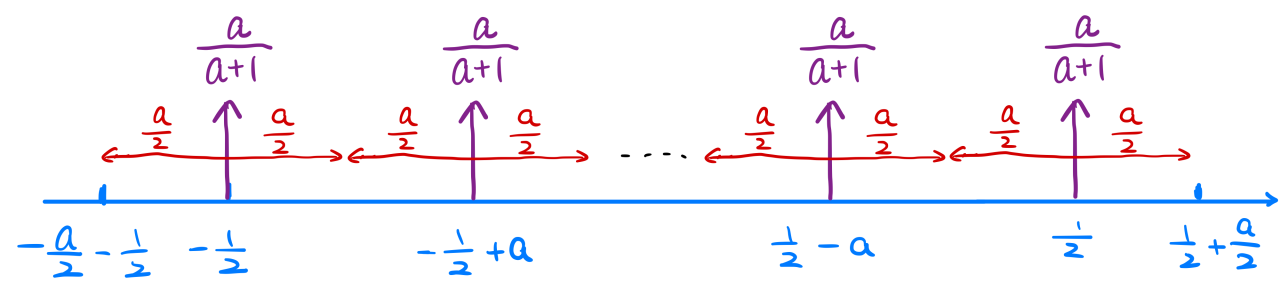
\includegraphics[width=\textwidth]{../range.png}
\end{figure}
We set $p(X=x)=\dfrac{a}{a+1}$, where $\mathcal{X}$ are the purple impulses signals in the figure. The red range represent that each $x\in\mathcal{X}=\{-\frac{1}{2},-\frac{1}{2}+\frac{a}{2},-\frac{1}{2}+\frac{3a}{2},\ldots,-\frac{1}{2}+\frac{a}{2}+i\cdot a,\ldots, \frac{1}{2}\}$ could cover to make $Y$ as uniform. \\
So in order to cover the full range in $[-\frac{a+1}{2},\frac{a+1}{2}]$, we have to has $a=\dfrac{1}{N}$, where $N\in \{1,2,\ldots\}$, and the capacity is $C=\max  \limits_{p(x)}I(X;Y)=\log(a+1)=\log\left(\frac{1}{N}+1\right) \ \text{bits}$.
And in other situations, $Y$ cannot be Unif$(-\frac{a+1}{2},\frac{a+1}{2})$ because in such strategy, $\mathcal{X}$ could not cover the full range $\left[-\frac{a+1}{2},\frac{a+1}{2}\right]$.

2. When $a>1$: \\
Wwe could see that when $y\in\left[\frac{1}{2}-\frac{a}{2},-\frac{1}{2}+\frac{a}{2}\right), f_Y(y)=\dfrac{1}{a}$, unless $\frac{1}{2}-\frac{a}{2}=-\frac{1}{2}+\frac{a}{2}\Rightarrow a=1$, it could be ignored, otherwise, $Y$ would never be Unif$\left(-\frac{a+1}{2},\frac{a+1}{2}\right)$. \\

So above all, we have proved that if and only if when $a=\dfrac{1}{N}, N\in\{1,2,\ldots\}$, the capacity of the channel is $\log\left(\frac{1}{N}+1\right) \ \text{bit}$. \\
And in other cases, we could not find a closed form solution for the $I(X;Y)$, so we need to use the Blahut-Arimoto algorithm mentioned in the text book $\S 10.8$.

\newpage